\documentclass[../main.tex]{subfiles}
\graphicspath{{\subfix{../img/}}}

\begin{document}

\newpage
\section{Projektmanagement}

\subsection{Risikomatrix} \label{risikomatrix}

Alle bekannten Risiken in Bezug zum Projekt sind in folgender Tabelle aufgelistet.
Dabei hat jedes Risiko folgende Attribute:
\begin{itemize}
    \item \textbf{Titel + Beschreibung}: Beschreibung des Risikos
    \item \textbf{Verantwortlich} Welche Gruppe dafür verantwortlich ist (INF=Informatik, MT=Maschinentechnik, ET=Elektrontechnik).
    \item \textbf{Kategorie}: In welcher Kategorie sich das Risiko befindet.
    \item \textbf{Ursachen}: Was passieren muss, damit das Risiko eintreffen kann.
    \item \textbf{Bewertung des Risikos}: Eintrittswahrscheinlichkeit, Auswirkung und Risiko Bewertung ohne Massnahmen
    \item \textbf{Massnahmen zur Risikominimierung}: Massnahmen um die Eintrittswahrscheinlichkeit oder Auswirkung zu minimieren.
    \item \textbf{Korrekturmassnahmen}: Was gemacht werden soll, wenn das Risiko trotzdem Eintrifft
    \item \textbf{Erfolgsfaktoren}: Beschreibt das Verhalten bei erfolgreicher Risikomitigation
    \item \textbf{Erneute Bewertung des Risikos}: Eintrittswahrscheinlichkeit, Auswirkung und Risiko Bewertung mit den definierten Massnahmen
\end{itemize}

Aus Darstellungsgründen wurden die Attribute der Risikos in zwei Reihen aufgeteilt. In der ersten Reihe werden die Risikos und ihre Auswirkungen genannt und bewertet, sowie die Verantwortlichkeit definiert. In der zweiten Reihe werden die Massnahmen zur Risikominderung, die Korrekturmassnahmen und die Erfolgsfaktoren genannt, weiter wird dazu nochmal eine Bewertung gemacht.

\begin{landscape}
\newpage
\scriptsize

\textbf{Legende:}
\hspace{1cm}
\textbf{VW:} Verantwortlich
\hspace{1cm}
\textbf{EW:} Eintrittswahrscheinlichkeit (1-5)
\hspace{1cm}
\textbf{AW:} Auswirkung (1-5)
\hspace{1cm}
\textbf{BW:} Bewertung (EW * AW)
\\
\vspace{1mm} \hspace{21.5mm}
\textbf{EWM:} EW mit Massnahmen (1-5)
\hspace{1cm}
\textbf{AWM:} AW mit Massnahmen  (1-5)
\hspace{1cm}
\textbf{BWM:} BW mit Massnahmen (EW * AW)


\renewcommand{\arraystretch}{1.5} % Adjust row height for readability
\begin{longtable}{|c|p{4.5cm}|p{5cm}|c|c|p{4.5cm}|c|c|c|}
\hline
\rowcolor{white}
& \textbf{Titel} & \textbf{Beschreibung} & & & \textbf{Ursachen} & \textbf{EW} & \textbf{AW} & \textbf{BW} \\ 
\cline{2-3} \cline{6-9}
\rowcolor{white}
\multirow{-2}{*}{\textbf{ID}}
& \textbf{Massnahmen Risikominderung} & \textbf{Korrekturmassnahmen} & \multirow{-2}{*}{\textbf{VW}} & \multirow{-2}{*}{\textbf{Kategorie}} & \textbf{Erfolgsfaktoren} & \textbf{EWM} & \textbf{AWM} & \textbf{BWM} \\ \hline
\endhead

\rowcolor[HTML]{F5F5F5} & Grip-Verlust normale Räder & Das Fahrzeug schleift über den Boden & MT & Mechanisch & Fahrzeug verliert Grip & 3 & 3 & 9
\\* \cline{2-3} \cline{6-9}
\rowcolor[HTML]{F5F5F5} \multirow{-2}{*}{R1} & Auf Mensaboden testen & Andere Räder/Geschwindigkeit anpassen & & & Fahrzeug hat Grip & 2 & 2 & 4 \\ \hline

\rowcolor{white} & Liniensensor falsche Daten & Der Liniensensor erkennt die Fugen als Führungslinie & ET+INF & Elektrisch & Fahrzeug folgt der Fuge & 4 & 4 & 16
\\* \cline{2-3} \cline{6-9}
\rowcolor{white} \multirow{-2}{*}{R2} & Kalibrierung des Sensors, Abgleich mit Kamera & Not-Aus verwenden & & & Fahrzeug folgt Führungslinie & 2 & 5 & 10 \\ \hline

\rowcolor[HTML]{F5F5F5} & Motorenposition ungenau & Für Rückstellen des Hindernis ungenau Positionswerte & ET & Elektrisch & Hindernis nicht innerhalb 2 cm & 3 & 3 & 9 \\* \cline{2-3} \cline{6-9}
\rowcolor[HTML]{F5F5F5} \multirow{-2}{*}{R3} & Langsame Fahrt bei Positionierung & Hallsensor, Drehgeber, Schrittmotor & & & Hindernis innerhalb der 2 cm Toleranz & 2 & 2 & 4 \\ \hline

\rowcolor{white} & Distanzmessung fehlerhafte Daten & Für die Erkennung der Distanz, des Hindernis, könnten falsche Messwerte eine ungewollte Aktion ausführen & ET & Elektrisch & Fahrzeug führt Hindernisbewältigung aus ohne ein Hindernis & 2 & 2 & 4 \\* \cline{2-3} \cline{6-9}
\rowcolor{white} \multirow{-2}{*}{R4} & Distanzwert muss längere Zeit konstant bleiben & Zweiter Sensor zum Vergleich verbauen & & & Fahrzeug führt Hindernisbewältigung nur bei einem Hindernis aus & 1 & 2 & 2 \\ \hline

\rowcolor[HTML]{F5F5F5} & Datenverlust & Verlust von Projektdaten/Forschungsergebnissen & INF & Projekt & Server offline & 2 & 5 & 10 \\* \cline{2-3} \cline{6-9}
\rowcolor[HTML]{F5F5F5} \multirow{-2}{*}{R5} & Regelmässige Backups erstellen & Daten aus Backups wiederherstellen & & & Daten sind zugänglich und schnell wiederherstellbar & 2 & 2 & 4 \\ \hline

\rowcolor{white} & Lieferschwierigkeiten & Teile, die bestellt werden haben Lieferverzögerung & ET+MT &  Market & Längere Lieferzeiten/Keine Lieferzeiten angegeben & 3 & 4 & 12 \\* \cline{2-3} \cline{6-9}
\rowcolor{white} \multirow{-2}{*}{R6} & Frühzeitig Bestellen, alternative Teile/Quellen suchen & bei alternativen Quellen bestellen & & & Teile können zeitnah verwendet verbaut werden & 3 & 3 & 9 \\ \hline

\rowcolor[HTML]{F5F5F5} & Software-Absturz & Software crasht während Einsatz & INF & Software & Prozess wird unerwartet beendet & 2 & 5 & 10 \\* \cline{2-3} \cline{6-9}
\rowcolor[HTML]{F5F5F5} \multirow{-2}{*}{R7} & Gutes Testen des Codes und Failsafe einbauen & Not-Aus verwenden & & & Fahrzeug kann nach Absturz von alleine wieder starten & 1 & 5 & 5 \\
\hline
\rowcolor{white} & Verlust Sensorkommunikation & Die Kommunikation zwischen Sensorik und Software ist gestört & ET+INF & Software & Fehlerhafte Daten oder fehlende Daten & 2 & 5 & 10 \\* \cline{2-3} \cline{6-9}
\rowcolor{white} \multirow{-2}{*}{R8} & Sicheres verbauen und Testen der Sensoren & Neueinstellung/Kalibrierung durchführen & & & Fahrzeug kann trotz fehlerhafter Sensordaten Aufgabe erfüllen & 2 & 3 & 6 \\ \hline

\pagebreak

\rowcolor[HTML]{F5F5F5} & Software zu anspruchsvoll für Computer & Die Leistung des Computers reicht nicht aus & INF & Software & Software-Lags, langsame Reaktionszeit & 3 & 4 & 12 \\* \cline{2-3} \cline{6-9}
\rowcolor[HTML]{F5F5F5} \multirow{-2}{*}{R9} & Software optimiert bauen & Langsamer fortsetzen & & & Fahrzeug kann trotz langsamer Laufzeit Aufgabe lösen & 3 & 3 & 9 \\ \hline
\rowcolor{white} & Pylone wird überfahren & Eine Pylone wird nicht erkannt & ET+INF & Elektrisch & Pylone wird nicht erkannt & 3 & 5 & 15 \\* \cline{2-3} \cline{6-9}
\rowcolor{white} \multirow{-2}{*}{R10} & Frühes Training und Testing & Not-Aus verwenden & & & Das Fahrzeug erkennt Pylonen & 1 & 5 & 5 \\ \hline

\rowcolor[HTML]{F5F5F5} & Unscharfe Bilder während Fahrt & Kamera liefert unscharfe Bilder & MT+INF & Software & Objekterkennung fehlerhaft & 4 & 4 & 16 \\* \cline{2-3} \cline{6-9}
\rowcolor[HTML]{F5F5F5} \multirow{-2}{*}{R11} & Bildaufnahme nur bei stehendem Fahrzeug & Fahrzeug stehen lassen & & & Das Fahrzeug erkennt Objekte korrekt & 2 & 4 & 8 \\ \hline

\rowcolor{white} & Fokus der Kamera & Fokus umfasst nicht benötigten Bereich & ET+INF & Elektrisch & Objekte werden nicht korrekt erkannt & 3 & 3 & 9 \\* \cline{2-3} \cline{6-9}
\rowcolor{white} \multirow{-2}{*}{R12} & Fokus-Range prüfen & Software anpassen & & & Fahrzeug erkennt Objekte & 2 & 2 & 4 \\ \hline

\rowcolor[HTML]{F5F5F5} & Grip-Verlust Omni/Mecanum & Fahrzeug verliert Grip bei Fugen & MT & Mechanisch & Fahrzeug verliert Grip & 4 & 4 & 16 \\* \cline{2-3} \cline{6-9}
\rowcolor[HTML]{F5F5F5} \multirow{-2}{*}{R13} & Testen der Räder & Mit Sensoren Position ausgleichen & & & Fahrzeug ist an gewünschter Position & 3 & 3 & 9 \\ \hline

\rowcolor{white} & Anzahl GPIO & Steuerung hat begrenzte Pins & ET & Elektrisch & Sensorinformationen nicht lesbar & 3 & 5 & 15 \\* \cline{2-3} \cline{6-9}
\rowcolor{white} \multirow{-2}{*}{R14} & Erweiterung mit Multiplexern & Alternative Schaltungen & & & Sensorinformationen verfügbar & 3 & 4 & 12 \\ \hline

\rowcolor[HTML]{F5F5F5} & Verschiebung bei Drehung & Keine genaue Drehung möglich & MT & Mechanisch & Fahrzeug schiebt seitlich & 3 & 5 & 15 \\* \cline{2-3} \cline{6-9}
\rowcolor[HTML]{F5F5F5} \multirow{-2}{*}{R15} & Testen & Zusatzfunktion abdocken & & & Fahrzeug dreht fix & 2 & 3 & 6 \\ \hline

\rowcolor{white} & Blendende Beleuchtung & Licht stört Kamera & ET & Elektrisch & Kamera sieht Blendung statt Objekt & 4 & 4 & 16 \\* \cline{2-3} \cline{6-9}
\rowcolor{white} \multirow{-2}{*}{R17} & LEDs vermeiden & Kameraeinstellung bei wenig Licht & & & Kamera erkennt Objekt trotz Blendung & 2 & 2 & 4 \\ \hline

\end{longtable}
\normalsize    
\end{landscape}

\newpage
TODO: Bild von Risikomatrix

Diese Risiken werden am Projektanfang möglichst minimiert. Dies kann beispielsweise anhand von Prototypen, geplanten Backup Lösungen oder vertieften Recherchen erfolgen.

\subsubsection{Recherche zu Risiko R16: Blendung der Kamera durch Reflexionen}
Um Reflexionen zu reduzieren, kann im Fotografikbereich mit Polarisationsfiltern gearbeitet werden, die nur Licht mit einer gewissen Polarisierung durchlassen. Mit Hilfe eines solchen Polarisationsfilters wurden Tests gemacht, um zu sehen, inwiefern die Reflexionen tatsächlich reduziert werden können. Dabei wurde darauf geachtet, dieselben Kamera-Einstellungen mit und ohne Polarisationsfilter zu verwenden.

\begin{table}[h!]
    \centering
    \begin{tabular}{|c|c|}
        \hline
        \parbox[c][1cm][c]{3cm}{\centering Ohne Polarisationsfilter} &
        \parbox[c][1cm][c]{3cm}{\centering Mit Polarisationsfilter} \\
        \hline
        \includegraphics[width=6cm,angle=90,origin=c]{img/polarisierungsfilter/pol4_n.jpg} & 
        \includegraphics[width=6cm,angle=90,origin=c]{img/polarisierungsfilter/pol4_j.jpg}  \\
        \hline 
        \includegraphics[width=6cm,angle=90,origin=c]{img/polarisierungsfilter/pol5_n.jpg} & 
        \includegraphics[width=6cm,angle=90,origin=c]{img/polarisierungsfilter/pol5_j.jpg} \\
        \hline
    \end{tabular}
    \caption{Vergleich Polarisationsfilter}
\end{table}

Die Resultate sind eindeutig. Bei gleichen Kamera-Einstellungen reduziert ein Polarisationsfilter die Reflexionen auf den Bodenplatten deutlich.


\addtocounter{subsection}{1}
\addcontentsline{toc}{subsection}{ 4.1   Projektplan}
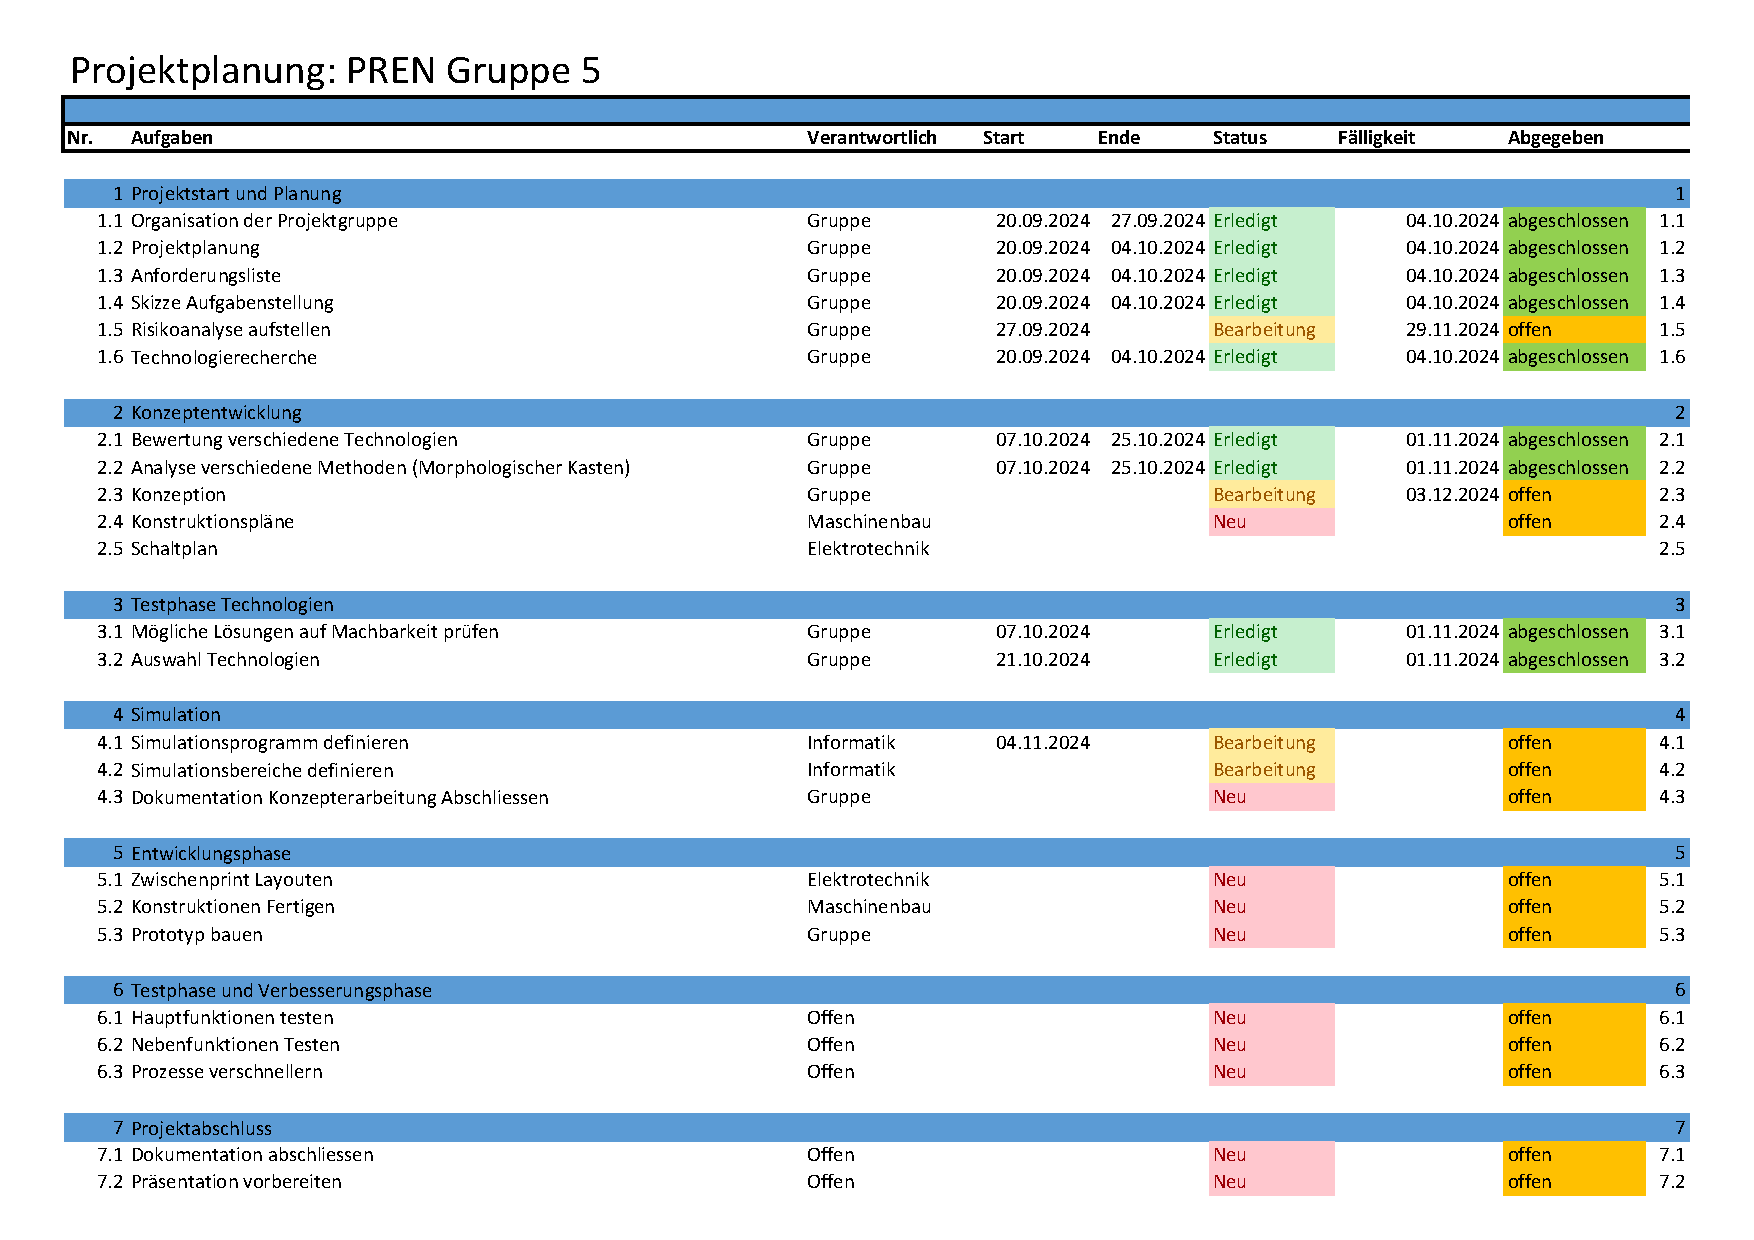
\includepdf[
  landscape=true,
  pages={1-},
  scale=0.9,
  pagecommand={\pagestyle{fancy}}
]{assets/Projektplan_v2.pdf}

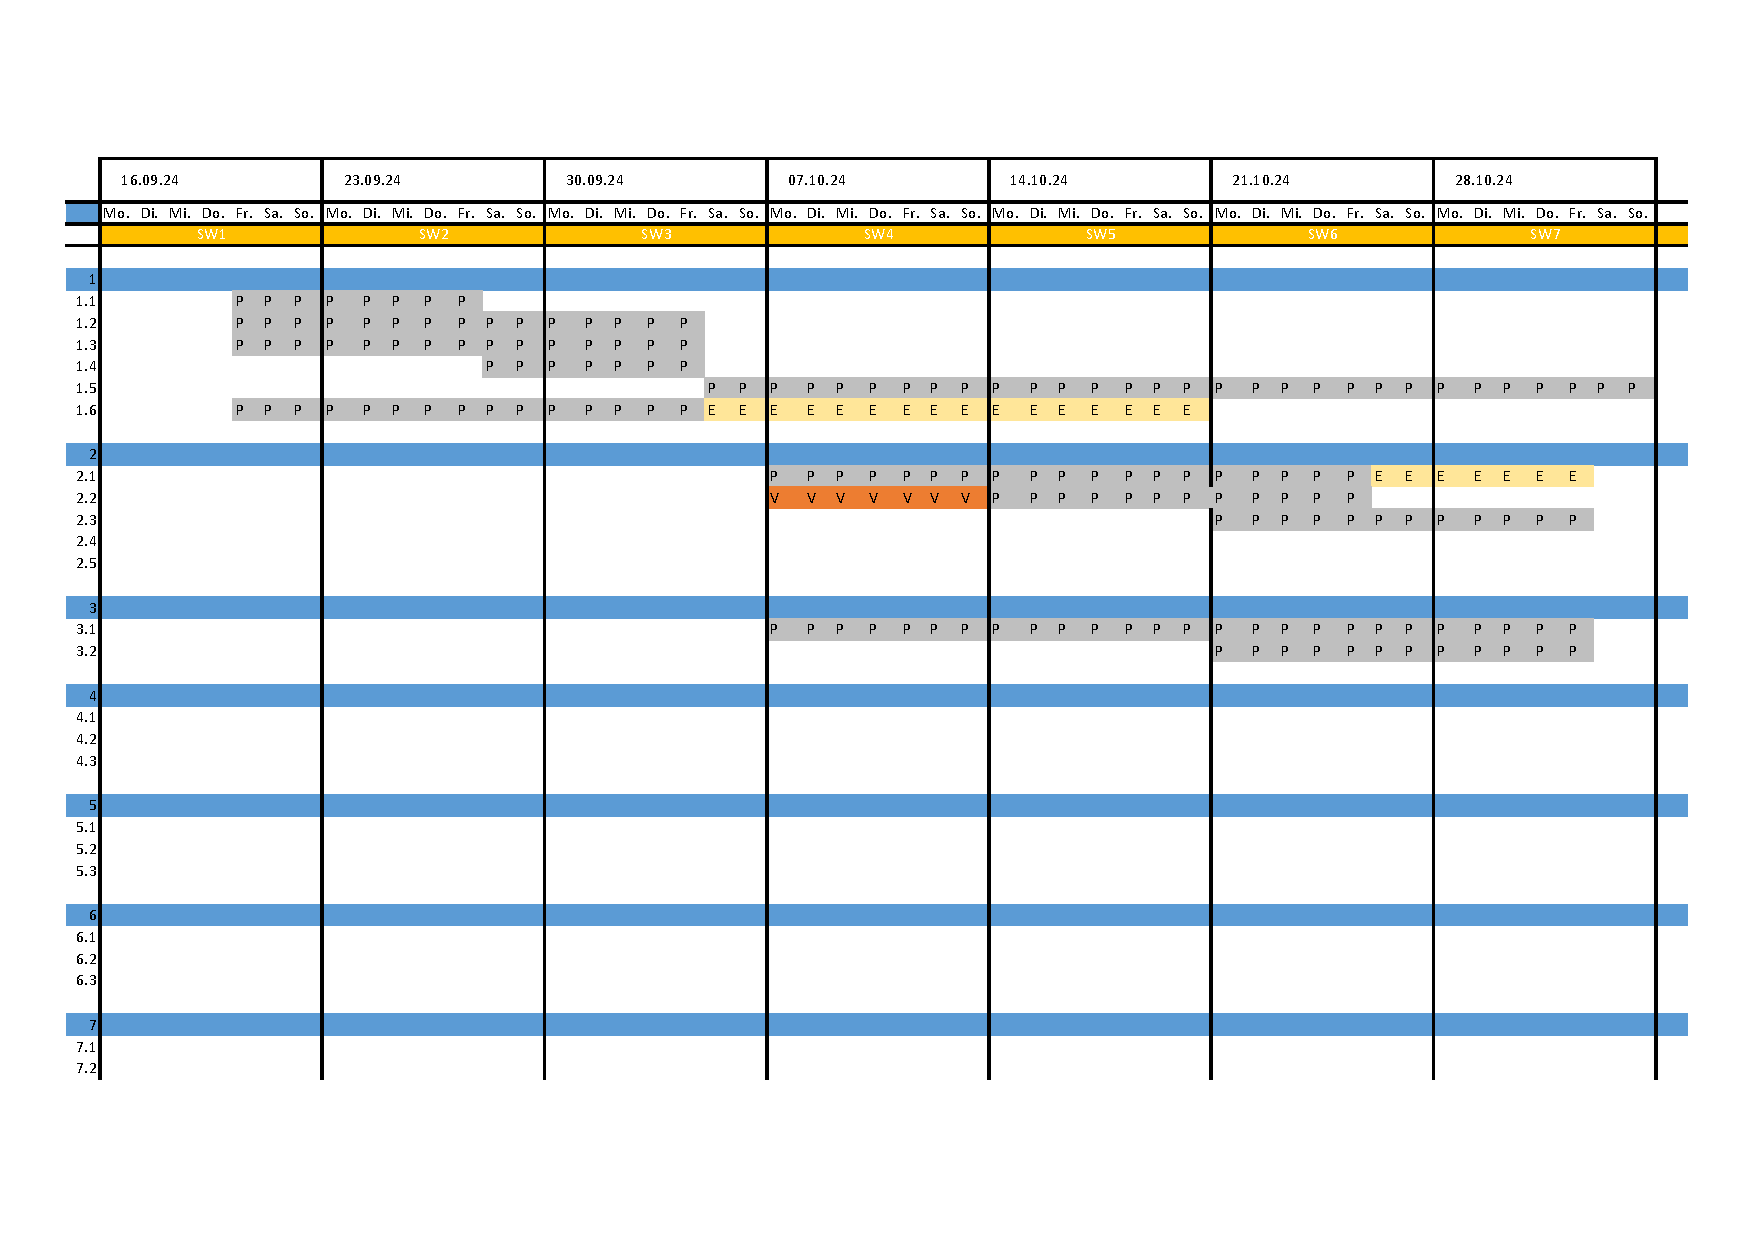
\includepdf[
  landscape=true,
  pages={1-},
  scale=0.9,
  pagecommand={\pagestyle{fancy}}
]{assets/Zeitplan_v2.pdf}
\end{document}